\chapter{Method}
\label{method}

In this chapter, I outline a general research program and associated substantive and experimental hypotheses. Following, I describe the use of Amazon Mechanical Turk for the collection of behavioral data, general procedure followed, and summary of the population sample observed.

\section{Research Program}
\label{researchprogram}

There is little question that interaction with computers change what we know and believe. Usability has long been concerned with the fit between user ``mental model'' and the design of user interfaces. Typically, such studies include the use of qualitative research techniques such as cognitive walk-throughs, eye-tracking, and card sorting. Such studies are often task-oriented and situated to address the use of specific products.

Dan Saffer, in his book \emph{Microinteractions}  \citeyearpar{Saffer:2013wn},  touches upon user interaction with user interface components, or features, that perform only one small task. For instance, a login screen embodies a self-contained interaction that may be quite small, but extremely important for user experience. This microinteraction has a clear start and end. As Saffer notes, some triggers to enter a microinteraction are user-initiated, and some may be system-initiated. Regardless, I believe there is a clear parallel to conversational discourse discussed in the previous chapter: users exchange information interactively.

This dissertation examines several microinteraction in the domain of online behavioral advertising. Of particular interest are phenomena relating to user confusion in the context of online interaction. 

The substantive hypothesis for questions asked in this dissertation is that \emph{some user confusion stemming from online behavioral advertising is caused by error in discourse understanding}. I contend that by regarding user interaction with graphical user interfaces as a form of discourse, we can account for some sorts of user confusion that may be difficult to see or may otherwise go un-noticed.

The next section summarizes specific research hypotheses for this dissertation. The research approach used to examine these hypotheses is \emph{randomized experimentatal}. The purpose for adopting such an approach is to determine causality for some sorts of user confusion. Each research hypothesis is paired to some aspect of discourse theory. Therefore, Chapters 5, 6, and 7 more fully motivate the connection between theory and practice prior to a presentation of results.

\section{Design of Experiments}
\label{designofexperiments}

The substantive hypothesis (user confusion stems from errors in discourse understanding) implies a set of research hypotheses, which in turn imply individual study hypotheses.

\begin{description}
\item[Research hypothesis 1:] \hfill \\ 
Graphical user interfaces have properties comparable to other forms of linguistic communication. 

\item[Research hypothesis 2:] \hfill \\
Graphical user interfaces can cause users to make faulty pragmatic inferences.

\item[Research hypothesis 3:] \hfill \\
A pragmatic inference derived while interacting with a graphical user interface may be affected when given immediate and direct feedback.
\end{description}

Each of the three sets of experiments described in Chapters 5-7 support one more more of the research hypotheses above. Specific research manipulations  are described below. The number in the left column refers to the experiment number.
\\
\\
\textbf{Research manipulation} (by experimental condition):
\begin{description}
\item[1A:]  \hspace{6pt}Suppose that pragmatic inference only occurs in linguistic (text or speech) interaction. A graphical user interface is used in the experimental condition whereas text is used in the control condition.
\item[1B:]  \hspace{6pt}Suppose that system feedback adds information to a situation model. Feedback is used in the experimental condition while none in the control condition.
\item[2A:]  \hspace{6pt}Suppose images and icons are objects that are both indexical. Images and icons are combined such that contrastive relations exist in the experimental condition while none exists in the control condition.
\item[2B:]  \hspace{6pt}Suppose advertising images are implicitly indexical. Explicit indexical element appears in the experimental condition while none exists in the control condition. 
\item[3:]  \hspace{12pt}Suppose that a user designs utterances taking into account potential listeners. Listener roles are explicit in the experimental condition while implied in the control condition.
\end{description}

Finally, the table below summarizes experimental designs. Each should be considered a pilot study. That is, experiments described are new and there are no other results against which to compare. The goal is to apply difference statistics to determine whether the variables described are independent (null hypothesis) or dependent. A relation between variables indicates some degree of predictiveness and causality. We can use information about causality to guide, or motivate, a strategy for reducing the possibility of miscommunication.

%% LyX 2.0.6 created this file.  For more info, see http://www.lyx.org/.
%% Do not edit unless you really know what you are doing.
%\documentclass[english]{article}
%\usepackage[T1]{fontenc}
%\usepackage[latin9]{inputenc}

%\makeatletter

%%%%%%%%%%%%%%%%%%%%%%%%%%%%%% LyX specific LaTeX commands.
%% Because html converters don't know tabularnewline
%\providecommand{\tabularnewline}{\\}

%\makeatother

%\usepackage{babel}
%\begin{document}
%B%
%\begin{table}
%\begin{center}
\begin{longtable}{l p{10cm}}
\caption{Experiment Design} \\
1A & 2x2x2 between group posttest-only design where the control group is
presented with a set of textual expressions and asked to answer
questions about their meaning. Treatment groups are presented with either textual expressions or a dialog box expressing the same set of choices and asked the same
questions. Independent Variables: Modality, Deontic force, Attitude
toward privacy. Dependent Variable: Pragmatic implicature\tabularnewline
\hline 
1B & Between group posttest-only design where two groups are presented
with a cookie banner and later asked about whether or not they believe
the website placed \textquotedbl{}cookies\textquotedbl{} in their
browser. The treatment group is presented with feedback about the
consequence of their action / non-action following presentation of
the banner. Independent Variable: Feedback. Dependent Variable: Pragmatic
implicature.\tabularnewline
\hline 
2A & Between group posttest-only design where five groups are presented
an advertisement in the context of a webpage and asked to identify
hyperlinks. Treatment groups are presented an advertisement with embedded
image icons at four levels (known icon + different company, unknown icon, known call-to-action (CTA), ``DAA opt-out icon'') while the control group is presented with an embedded image from the same company as the advertiser. Independent
Variable: Icon type. Dependent Variable: Indexicality of icon. \tabularnewline
\hline 
2B & Between groups posttest-only design where three groups are presented
an advertisement in the context of a webpage and asked to identify
hyperlinks. Treatment groups are presented an advertisement at two
levels (iconic CTA, textual CTA) while the control group is presented
with an advertisement with no CTA. Independent Variable: Modality
of CTA. Dependent Variable: Click target.\tabularnewline
\hline 
3 & Between group repeated measures posttest-only design where a control
group is asked to respond to a survey containing questions relating
to activities (using questions drawn from \cite*{Acquisti:2012tp}; embarrassing, socially / ethically questionable, illegal). Participants
are notified in a privacy statement that there may be ad trackers
on the site. The treatment group receives exactly the same notification
and survey. However, tracker presence is indicated in a visual display
throughout the participant's session. Independent Variable: Visual
presence. Dependent Variable: Propensity to respond in the affirmative
to engaging in specific behaviors.\tabularnewline
\hline 
\end{longtable}
%\end{center}
%\end{table}
%\end{document}


Of course, not every usability problem needs be tested using experimental methods. But there are two good reasons to do so here:

\begin{sloppier}
\begin{enumerate}
\item No causality has yet been determined for presumed cases of mis-communication studied here. In fact, it may not even be apparent that there is a problem at all.
\item Though linguistic theory offers explanation for the sort of miscommunication described in experiments here, there are no earlier studies with which to compare. This dissertation intends to make such a relation clear and provide a path for future exploration. 
\end{enumerate}
\end{sloppier}

Each of the research hypotheses above has bearing on current practice in online behavioral advertising as represented in technical specifications of existing or proposed standards. Though self-regulatory bodies for OBA suggest that specific principles are adhered, effectiveness is in question. Marketing advocates affirm that self-regulatory practices are effective  \citep{AdChoicesOurExpe:2012ux}.  However, research studies by policy advocates  \citep[e.g.,][]{Komanduri:2012wo,Mayer:2012wt}  have raised issues of industry non-compliance. Even if compliance were universal, usability studies have uncovered inadequacies in terms of communicative efficacy  \citep{Leon:2012vu,Ur:2012ws,Hastak:2010vf}.  The benefit of the approach in this dissertation is the ability to test technical specifications, and ascertain effectiveness in context. 

One of the particular challenges of the randomized experimental approach is the need for a larger number of participants than one might expect from a traditional usability experiment. Increasingly, psychologists and linguists have come to rely on the large pool of volunteers available via the Amazon Mechanical Turk (AMT) crowdsourcing platform. The next section addresses both advantages and disadvantages of AMT for experimentation. Characteristics of the user sample studied have particular bearing on the research validity of experiments presented in this thesis.


\section[Mechanical Turk]{Mechanical Turk as a Platform for Human Intelligence Tasks}
\label{mechanicalturkasaplatformforhumanintelligencetasks}


The original Mechanical Turk constructed in the 18th century was a hoax. In all appearance, he was a mechanical man dressed in an turban and robe, seated behind a large cabinet. Despite being mechanical, he played chess like no other machine could. Of course, unknown to most at the time, inside the cabinet was a tiny space where a real human played the game by controlling the automaton's arms on the chessboard. 

By contrast, Amazon's Mechanical Turk (AMT) is no hoax. From a simple command line interface, requester's can create ``human intelligence tasks'' and farm them out to a sea of workers. Within seconds, a task may be accepted, completed, and remunerated without the requester ever knowing or communicating with the invisible worker. AMT shares a simple design concept with the original Turk: a human is in the machine. The idea is a ``job posting board'' where human intelligence is needed. Any of a variety of ``Human Intelligence Tasks'' (HITs) can be posted along with small monetary rewards ranging from cents to dollars. AMT is a prototypical example of crowdsourcing --- outsourcing to a large, undefined community of people (i.e., crowd).

\subsection{The AMT Marketplace}
\label{theamtmarketplace}

In 2006, Wired magazine published the influential \emph{The Rise of Crowdsourcing}  \citep{Howe:2006uj},  which tells the story of the rise of the amateur on the web. Highlighted, is the example of a stock photo site iStockphoto which created a marketplace for amateur photographers. Professional grade camera technology at affordable prices combined with the ability to upload content to the Internet, search and categorization, and micro-payments changed the market for photographers and photo purchasers. Over the last decade, the power of many users over distributed networks has changed the world. Today, FaceBook and eBay could not exist without the contributions of their users.

The irony is, of course, that by engaging in the creation of user-generated content on the web, people have become part of the machine. This has led to the well-known technology humanist Jaron Lanier to rail against the de-humanization of the web. His position is --- to design applications that treat humans as machines devalues both people and content ``making ourselves into idiots''  \citep{Lanier:2006wb}.  Lanier particularly dislikes Wikipedia which creates a false sense of authority behind information by removing any connection between the real author of the information as well as a subjective context for the interpretation of content  \citep{Lanier:2010ud}. 

Nevertheless, crowdsourcing has become a viable economic model on the web. More than a million workers login to crowdsourcing platforms to complete short tasks for pay-per-task compensation  \citep{Munro:2011tm}.  And who is the invisible worker? As reported on The Mechanical Turk Blog in August of 2012, ``turkers'' comprise a workforce approximately 500,000 persons (at any one time) across 190 countries. In an analysis of the AMT marketplace over multiple studies,  \cite{Mason:2011cl}  report that the majority of turkers reside in the United States or India and tend more likely to be female (55\%) with a median average age of 30 and, on average, earning 30K per year. According to Ipeirotis  \citeyearpar{Ipeirotis:2010tt,Ipeirotis:2010jo},  workers in the US are more likely to use AMT as a secondary source of income while those in India use it as a primary source of income. Workers are self-selected on the marketplace, working for cash payments in US dollars and Indian rupees. All studies agree that workers are represented across a wide range of ages, ethnicities, countries, languages and income.

The AMT marketplace has been active since 2005. Among the most well-known documented instances of use, turkers were asked to help search through sections of satellite imagery to flag images with anomalies. The hope was that turkers might be able to help pinpoint the 2007 crash site of aviator Steve Fossett. This event so permeated the media at the time, I signed up to become a turker in order to participate. In the end, Fossett was not found in the region examined by turkers. In fact, there was some criticism toward the use of turkers for annotating satellite imagery. With little understanding of what constitutes anomaly in satellite imagery, the usefulness of generated leads were considered by some to be questionable.

Since then, AMT has been used for a variety of tasks, some of which call for specific skill or expertise, such as knowledge of a foreign language. More common are tasks that involve transcription, rating, editing, and image annotation. The AMT website provides a basic web interface for loading HITs, though it is also possible for requesters to direct workers to an external website or directly embed that website as an iframe on the AMT site.

\begin{figure}
\centerline{
  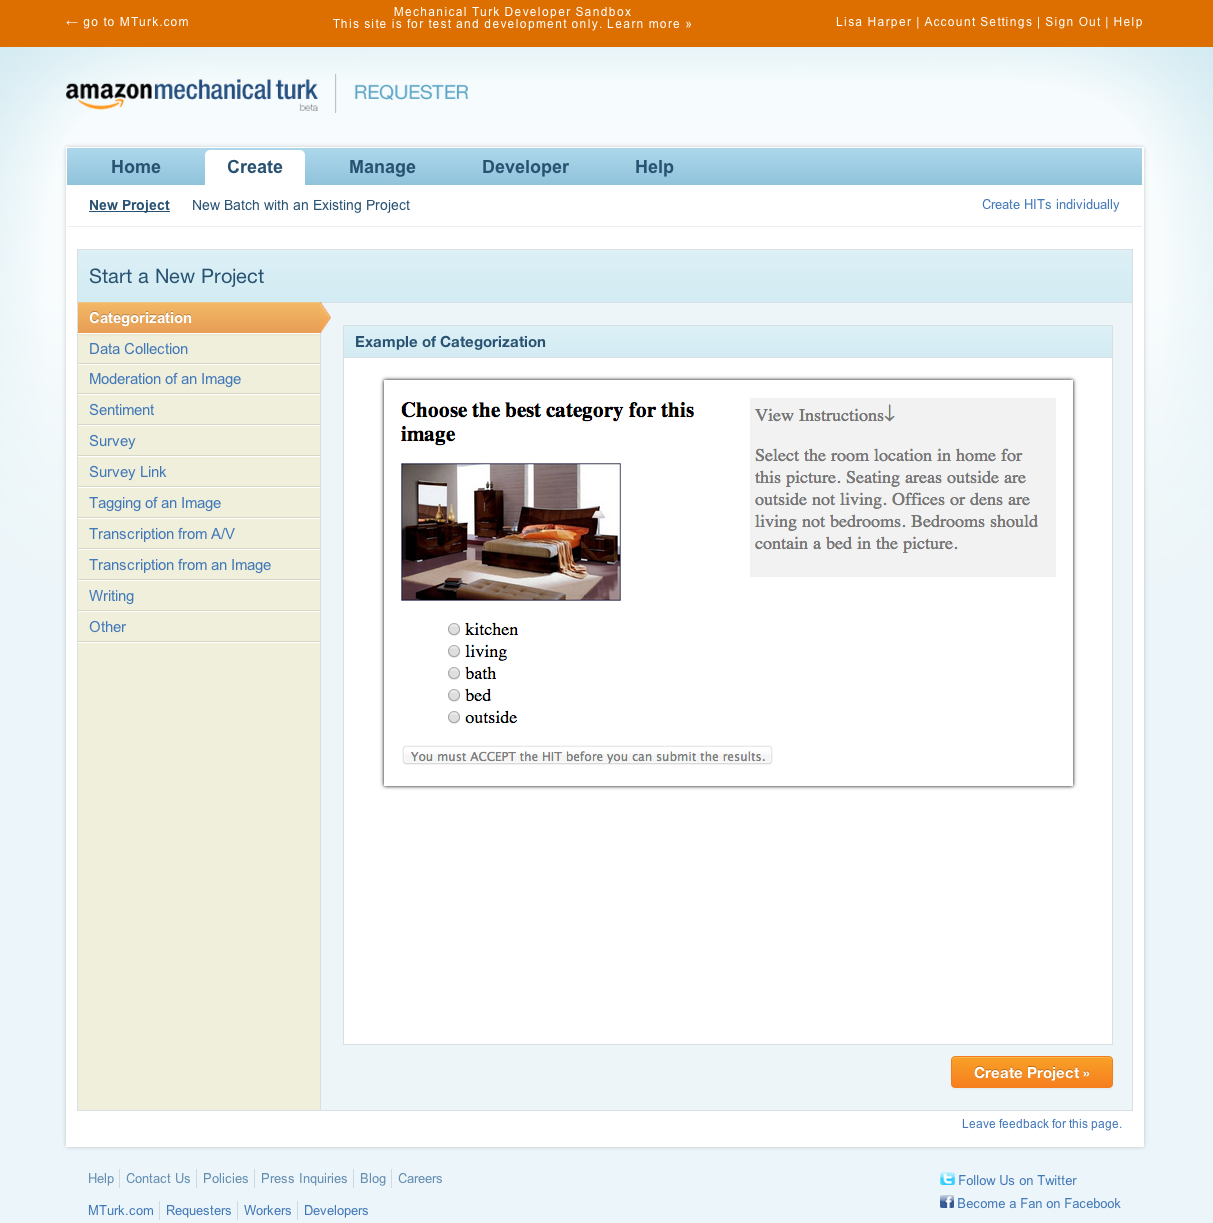
\includegraphics[scale=.5]{chapter4.tex/amt-creator}
  }
\caption{AMT Requester Website}
\label{requestor}
\end{figure}

Workers themselves comprise a community that interact on public forums, such as \emph{Turker Nation}, and through networks such as Twitter. Once on the AMT website, workers track their earnings (managed by Amazon), status (HIT success), qualifications, and the ever revolving database of available tasks.  \autoref{requestor}  is a screengrab taken from the AMT developer sandbox, a place for requesters to test tasks before deploying on the AMT website.

\begin{figure}
\centerline{
  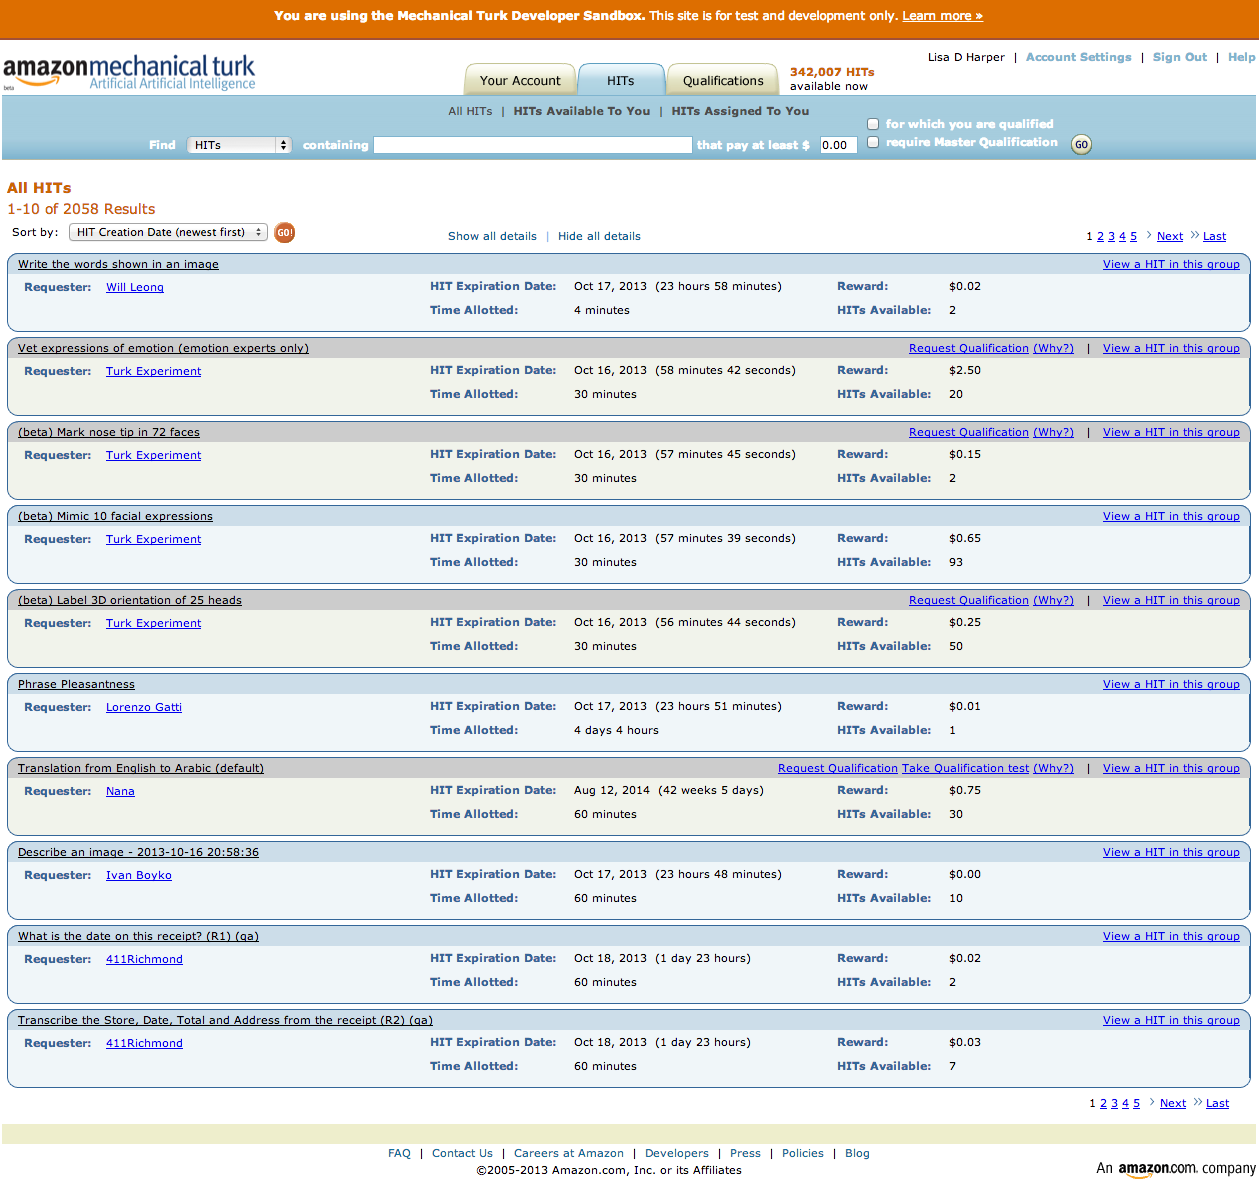
\includegraphics[scale=.5]{chapter4.tex/worker-hits}
  }
\caption{AMT Worker HITs}
\label{worker}
\end{figure}


Requesters define the task, number of tasks available, payment, qualification, and expiration date. Requesters must provide a validated US bank account and address in order to initiate tasks. Some basic worker qualification types are provided by Amazon out-of-the-box: worker HIT success and demographic region are commonly used by requesters. However, requesters also use qualifications as a mechanism for training workers. By requiring workers to ``train'' and go through testing, workers with special skills may be utilized in future tasks.

Because the worker success metric is often used as a filter for ensuring higher quality work --- and as a means for obtaining higher paid HITS --- workers take care to protect their rating. This means that requesters are also held accountable in their dealings with workers, via informal ratings over social media channels. Though some HITs may be paid automatically, it is fairly common for requesters to do quality control before accepting HITs. HIT rejection has negative consequences and is not taken lightly by the turkers.

There are a number of obvious advantages to using AMT. The workforce is roughly half a million strong and available around the clock. They represent a wide demographic range, many quite well educated. Amazon manages and automates payments and ensures the pool of workers abides by its terms of use.  \cite{Mason:2011cl}  observed that, for experimental research, a key advantage is faster iteration between hypothesis formulation and testing. However, there exists a number of real concerns and issues with crowdsourced experimentation. These are discussed below.

\subsection{General Concerns with the Use of AMT for Experimental Research}
\label{generalconcernswiththeuseofamtforexperimentalresearch}

First, and foremost, AMT is an Internet-based platform.  \cite{Reips:2006bm}  noted advantages as well as disadvantages to experimentation over the Internet (relative to the first four bullet points below). However, there are also number of other issues particular to Mechanical Turk.

\begin{enumerate}
\item \textbf{User Fraud.} There is the possibility of worker "gaming" through multiple submissions. The Turk Requester's Blog \footnote{\url{http://turkrequesters.blogspot.com/2013/01/the-reasons-why-amazon-mechanical-turk.html}} gives an example from the Romanian Mturk Forum, in which on every page (on a total of more than 300), are discussions of how to break Amazon's terms of service. As a result, Amazon adjusted their policy to an invitation-only registration for International workers \citep{Chiarella:2013vz}.
\item \textbf{Self-Selection.} Users self-select by reviewing titles, payment, time expected, and instructions. Unless controlled, users are generally able to preview eternal websites (or embedded iframes) to decide whether they wish to accept a given HIT. 
\item \textbf{Drop-outs.} AMT workers have the ability to return or abandon HITs without affecting their reputation. However, requester's don't automatically see which workers accept --- though don't complete --- assignments, so its difficult to gauge dropouts. 
\item \textbf{Mis-communication.} Reduced communication between requesters and workers may mean that directions are not well understood or followed. This can be difficult to detect and debug.

\item \textbf{Screening.} Amazon provides no general mechanism for screening aside from a general mechanism for filtering via qualifications. Of note, is the need to screen for demographic criteria and prior participation. This study has the particular need for the latter: excluding workers who have participated in one experiment from participating in another.  The mechanism that AMT provides is exclusion by assignment:  once a worker has accepted an assignment, that particular assignment is no longer available. For example, Experiment 2A of this dissertation required at least 300 subjects. Once a worker accepted this HIT the other 299 assignments were no longer available. But, without cross-experimental controls, it would be possible for some worker to accept a HIT from a closely related experiment, potentially biasing results.
\begin{sloppier}
\item \textbf{Compensation.} The very fact that AMT is fee-based places obligation on both the requester and worker. \cite{Mason:2009dr} investigated the relationship between compensation and performance in two experiments on AMT. They observed no interaction between difficulty of task and compensation on performance. They also found that increasing compensation alone did not improve accuracy. But how workers were paid (pay-per-word, pay-per-puzzle) did have an impact on output and accuracy. 
\end{sloppier}
While it is common for workers to accept tasks for pennies each, some workers find by working many low paying tasks in quick succession, they are able to earn close to minimum wage.\footnote{See discussion at \url{http://mturkforum.com/showthread.php?2744-How-much-do-you-earn-per-hour}, for example.} More typically they earn much less \citep{Paolacci:2010ws}. Though most workers appear attracted by the earnings potential, others participate for reasons such as boredom, fun, curiosity, and even education \citep{Behrend:2011dx}.

The studies in this dissertation limit participation to workers with a high HIT acceptance rate. From discussion on turker forums and blogs (e.g., \textit{Turker Nation}, \textit{mTurk Forum}, and \textit{Turkkit-Reddit}), its clear that these workers expect to be paid more than other workers. And many take this work quite seriously. 

\item \textbf{Quality and Reliability.} Beyond recruiting from the most reliable workers available, how much should quality be of concern? From prior crowdsourcing experiments on Amazon Mechanical Turk (AMT), quality is a valid concern \citep{CallisonBurch:2010vk,gormley-EtAl:2010:MTURK}. In a study of translation tasks, researchers consistently receive poor and noisy translations including blank annotations, misspellings, copy-pasting of machine translations, and downright cheating \citep{Ambati:2010ud}. Having workflows for the filtering of noisy data has proven vital in this environment. However, it is feasible to filter noisy judgements of non-experts depending on the task: in an image annotation task \cite{Nowak:2010gt} found that, while agreement between experts and non-experts varies depending on the measure used, its influence on image ranking as a whole, is minimal. Other sorts of studies echo this finding including labeling text with emotion \citep{Snow:2008wo}, search relevance judgements \citep{Alonso:2009vya}, and more.

\item \textbf{Presentation Consistency.} All Internet experiments conducted in the wild suffer the need for exceptional attention to cross-browser effects and robust services. If the experiment relies on everyone being able to see stimuli at the same resolution and in the same manner, then both scripts and screens need to be tested carefully, both across platforms and browsers. Furthermore, hosted services require reliable access by hundreds simultaneously --- and with little risk of downtime.

\item \textbf{Anonymity.} Finally, though we would like to believe that the human in the machine is anonymous, reality differs. It is estimated that 50\% of workers have been linked to public Amazon user profiles \citep{Lease:2013vq}. This means that Amazon worker Ids are essentially PII. And, in fact, many workers are not blind to this.
\begin{sloppier}
\item \textbf{The "Superturker".} Legal scholar Dan Kahan warns particularly of a side-effect of prior, repeated exposure to cognitive studies on AMT \citep{kahan:2013blog}. Chandler, Mueller, and Paolacci \citeyearpar{Chandler:2013bw} note that while the probability that any one worker has seen some manipulation, there is a population of "superturkers" (prolific workers) who are significantly more likely to end up in studies. Pooling 16,408 HITs in 132 unique studies, they found that HITs were completed by 7498 unique workers. The top 10\% of prolific workers completed 41\% of total HITs. On a positive note, \cite{Chandler:2013bw} note that these turkers are less likely to be multi-tasking and more likely to be available for follow-up studies such as required for longitudinal research. On the negative side, these workers are much more likely to have participated in cognitive tasks potentially biasing them for future cognitive tasks \citep{Chandler:2013bw}.
\end{sloppier}
\end{enumerate}


\section{General Procedure}
\label{generalprocedure}

Each experiment in this dissertation was delivered over the Internet in a web browser. Subjects (AMT workers) were randomly assigned to groups per study design. Experiments were implemented within a Qualtrics ( \url{http://qualtrics.com} ) survey using supplementary, custom JavaScript\slash HTML\slash CSS code that I wrote, as needed. Surveys were accessible via an HTTPS encrypted iframe on the AMT website ( \url{https://www.mturk.com}). 

In order to participate, AMT workers selected my HIT from a worker queue  (\autoref{worker}).  Three base qualifications were stipulated:

\begin{sloppier}
\begin{itemize}
\item workers must be 18 years or older (provided by the Amazon Mechanical Turk Terms of Service in \autoref{amazon});
\item workers must be physically located in the United States; and,
\item Workers must have a HIT success rate of 90\% or better. 
\end{itemize}
\end{sloppier}

The AMT API provided for qualification criteria such as geographic region and HIT success rate. By specifying these as requirements, Amazon automatically matched eligible workers to my ``surveys''. A sample assignment (Experiment 1A) is provided in  \autoref{assignment}. 

Using AMT command line tools, I tested each experiment in the AMT sandbox before deploying to AMT. Requesters can monitor assignment progress, approve or reject workers, download results, and assign bonuses from their dashboard. I tested assignments in several browsers both on on a Mac and Windows PC to ensure functionality and appearance were consistent. Following successful tests, I pushed assignments to AMT. 

Workers who selected one of my HITS were told they would be participating in either a language study, user interface study, image annotation study, or ethics survey, depending on the experiment. Because these were all studies of language use, workers were expected to have basic \emph{linguistic competence} in English. It was assumed that if they were on the Internet capable of responding to a request to participate in an online experiment, and residing in the United States, they had adequate competence in English. However, I also provided a demographic survey question targeting fluency level, if the subject was not a native speaker of English.

\begin{sloppier}
Each experimental design was deployed as a single Qualtrics survey. Qualtrics provides for sophisticated functionality such as survey flow, block randomization, display and question logic, and a JavaScript application programming interface (API). Several of my surveys required hand-coded instrumentation not provided by Qualtrics. I  discuss instrumentation in the methods section of each experiment described.
\end{sloppier}

Because I conducted multiple, related experiments simultaneously, exposure to one experiment potentially disqualified a worker from other experiments. For example, Experiment 1A has a potential priming effect on the topic of Internet privacy that could potentially bias that same worker in Experiment 1B. In such cases, I included a message on the preview that said something like, ``please don't accept this HIT if you have previously participated in an experiment with a blue rectangle.'' As reinforcement, I checked each worker on acceptance of consent against a database of prior workers. If a worker had already participated in a closely related experiment, a message was presented to that worker to please return the HIT. Then they were prohibited from further access. Eve so, it was still possible for a single worker to participate in more than one experiment. For example, if a worker signed up for Experiment 1B, they were allowed to also sign up for 2B. 

In each experiment, workers previewed basic instructions  (\autoref{instructions})  before selecting the HIT. I inserted custom code to prevent participants from advancing beyond this screen until the HIT had been accepted. In order to proceed, the worker must have clicked ``Accept HIT''.


\begin{figure}
\centerline{
  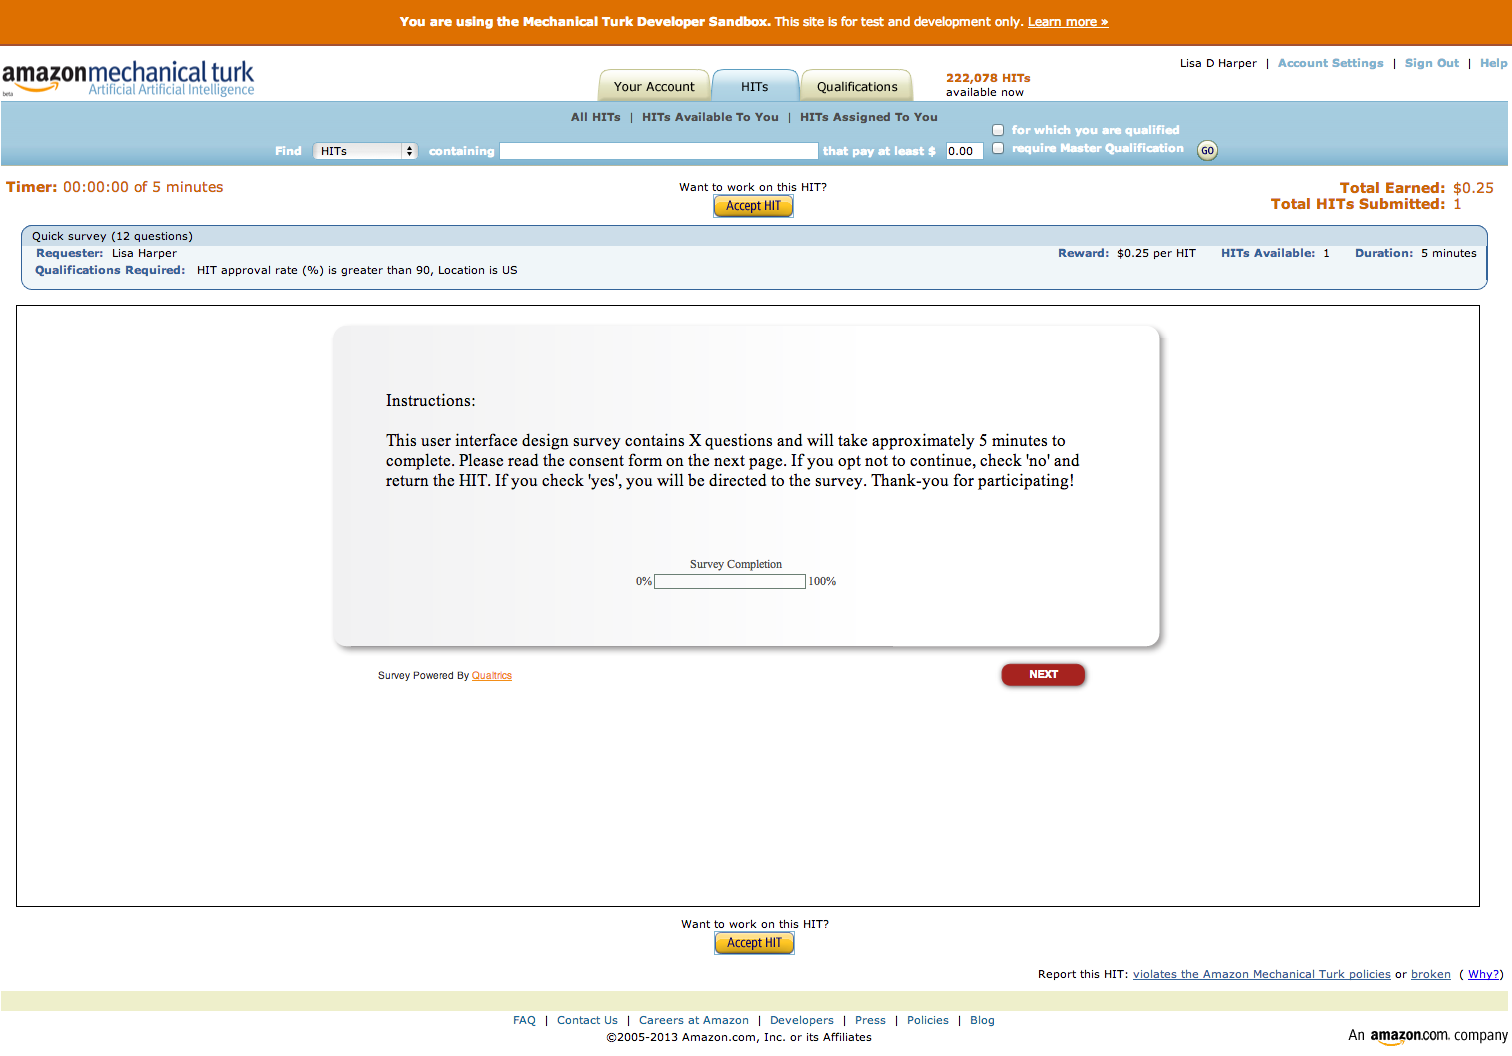
\includegraphics[scale=.4]{chapter4.tex/instructions}
  }
\caption{Participant Instructions (Experiment Three)}
\label{instructions}
\end{figure}


After clicking ``next'', a consent form was displayed (see  \autoref{consent}).  Again, in order to continue, the participant must have selected ``yes'' to continue.

General experiment flow is depicted below  (\autoref{flow}). 


\begin{figure}
\centerline{
  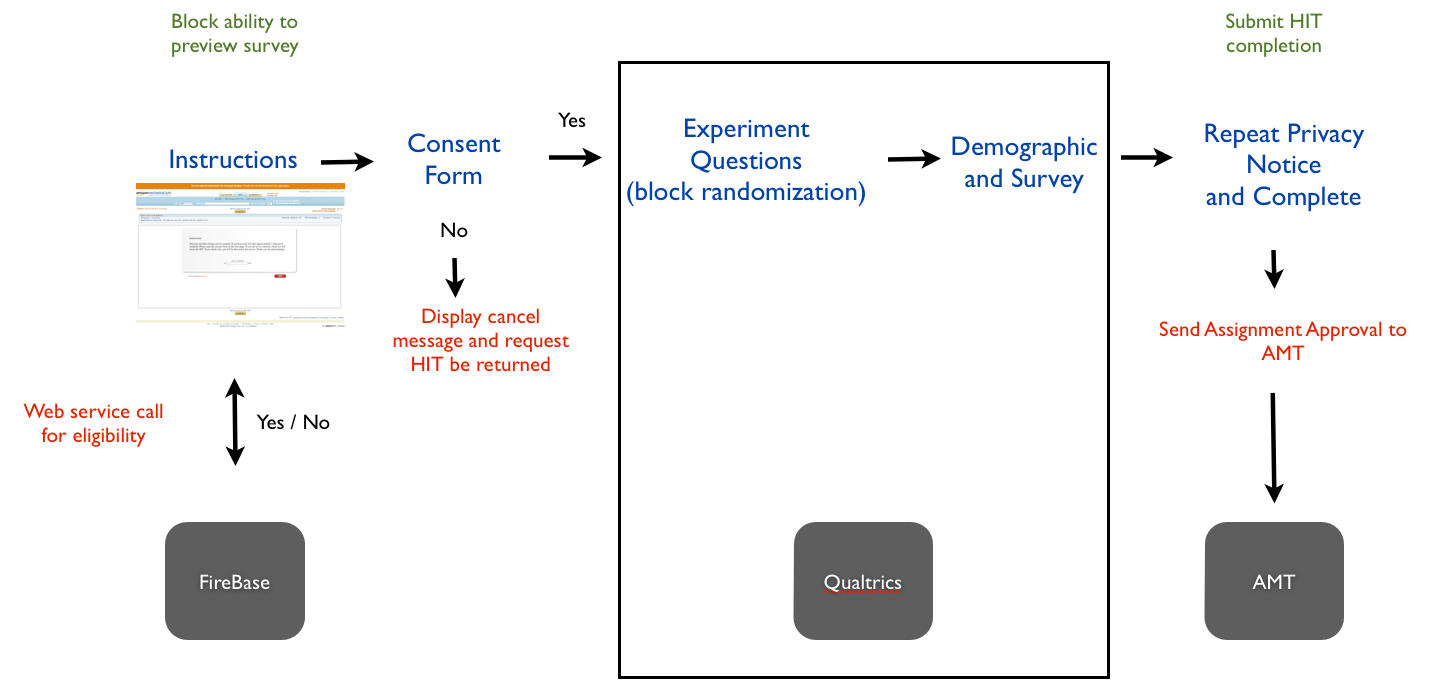
\includegraphics[scale=.25]{chapter4.tex/expflow}
  }
\caption{Experiment Flow}
\label{flow}
\end{figure}


At the completion of each survey, I configured assignments to automatically approve HITS so that Amazon would pay the worker immediately. Experiments were designed to take approximately three minutes to complete. I offered 15 cents for most. While it was also possible to manually review results before approving HITs, I decided this was not necessary for any of the studies included here since workers were recruited from those with known high performance. I did, however, manually assign random dollar bonuses after assignment completion.

\section{Data Storage and Privacy}
\label{datastorageandprivacy}

Data was stored in three places  (\autoref{data-storage}): AMT, Qualtrics, and FireBase.  AMT stored a list of workerIds for each experiment, Qualtrics stored survey data (but no workerIds), and FireBase was used to store a list of worker hashes (but no data or workerIds).

\begin{table}
\caption[Data Captured]{Data Captured}
\label{data-storage}
\centering
\begin{tabular}{cp{7cm}}
\toprule
Stored & Type of Data\tabularnewline
\hline 
Amazon Server \medskip{} & WorkerId, AssignmentId, HitId, Accept / Reject, Fees paid\tabularnewline
Qualtrics Server \medskip{}  
 & Random number identifier, Experiment data\tabularnewline
FireBase Server\medskip{}
 & Hash of workerIds for each experiment\tabularnewline
\end{tabular}
\end{table}

There was no connection between AMT and Qualtrics except for URL-encoded data passed to and from the Qualtrics server:

\begin{itemize}
\item On acceptance of a HIT, Amazon passed Qualtrics an AssignmentId, HitId, and WorkerId. 
\item On completion of the HIT, Qualtrics sent back to Amazon the AssignmentId. 
\end{itemize}

Survey data was not stored on Amazon's servers nor was participant identity accessible to Qualtrics via the AMT API. Because AMT does not offer ``verified'' user profiles, users can lie about their demographic group to qualify for a study. However, given the relative anonymity of the system, most appear to be honest  \citep{Ipeirotis:2010jo}.  

The Firebase service listed above was required only to disqualify workers from participating in certain experiment combinations. To safeguard identity, my code on Qualtrics converted the AMT WorkerId to a 32-bit hash and passed this hash to the Firebase service. New prospective workerIds were hashed and compared with the hash list on the Firebase service. Hashing is uni-directional, thus it is not possible to recover the original WorkerId from a hash list alone. 

On Qualtrics, the WorkerId was discarded and replaced with a random number identifier. WorkerId was treated as Personally Identifiable Information (PII) and de-linked from the data such that it would not be possible to re-link workerIDs to experiment results. Furthermore, though Qualtrics retains IP address data by default, I turned this, and other browser identifiers, off for these experiments. Because no identifying questions were asked, nor was IP address collected, all experiment data collected is fully anonymized. 

The next section addresses characteristics of the population sampled.

\section{Population Sample}
\label{populationsample}

The first and third columns of the table in  \autoref{survey-response}  summarize questionnaire responses across the five studies described in Chapters 5 - 7. Of the 1158 subjects who took the demographic survey, 84\% were unique, with 16\% duplication due to participation in more than one experiment. This was possible, depending on the order in which workers accepted tasks. For example, if a worker accepted a HIT in Experiment 3, that same worker was later still eligible for any of the other experiments. However, once participating in Experiment 1B, he or she would have been no longer eligible to participate further.

Demographics are comparable to those published in other studies  \citep{Ross:2010jm,Ipeirotis:2010tt,Mason:2011cl}, though the sample I collected was skewed more toward males.  Of 1158 subjects, 73\% were under 35, 53\% male, 73\% caucasian, 97\% English speaking, 86\% having at least some college, and 53\% making under 30,000 per year. The profile drawn here is from a set of workers with a 90\% or better HIT acceptance rate and from the United States.

In September of 2011,  \cite{McDonald:2011uv}  conducted a user survey on AMT to study the differences between what users expect ``Do Not Track'' to mean versus DNT definitions under debate. At the time, DNT was very new. They studied 304 participants limiting participation to the United States. 81\% had never heard of DNT.

Though I did not use those exact questions in my survey, in October of 2013, 91\% reportedly knew what a tracking cookie is. 73\% admitted to using browser plugins for privacy protection and more than half to configuring their browsers to ``opt-out''. However, despite that AMT workers are much more knowledgeable than two years ago, most still do not realize that DNT, as specified by advertisers, is limited to not showing targeted advertisements: information is still collected, stored, and used.

In an older study (not on AMT),  \cite{Acquisti:2005hv}  found a correlation between concern for privacy and income. Those with higher incomes were generally more concerned with privacy. However, this may have correlated more strongly with knowledge than income. They noted that their sample particularly lacked knowledge about technological or legal forms of privacy protection.

\section{Validity}
\label{validity}

Discussed below are three aspects of validity for studies using Mechanical Turk: internal, external, and construct validity. Questions of statistical validity are addressed in the results sections of experiments.

\subsection{Internal Validity}
\label{internalvalidity}

Internal validity concerns the equivalence between groups and the control of extraneous variables. Other behavioral experiments utilizing AMT  \citep{Crump:2013fn}  have suggested that the pool of available workers is sufficiently representative and large such that random assignments consistently produce results equivalent to those produced in carefully controlled laboratory settings. Furthermore, it is possible to conduct experiments where workers may are not aware that they are in an experiment (one source of experimental bias). Also, Paolacci et al.  \citep{Paolacci:2010ws}  found that retention was particularly high on AMT, compared to other pools compared (university student population and Internet boards). However, they noted that, unlike student populations, turker membership is organic and workers may be potentially available for years. This particularly highlights the need to track responses across experiments.

More insidious to internal validity may be the effects of payment itself. Two effects of \emph{volunteer bias} are of particular concern are: 1) effect of informed consent; and 2) effects of obligation incurred by accepting a HIT and, as as result, payment for services.  \cite{Rush:1978tw}  found difference between unpaid volunteers and paid subjects in a selective attention task. Unpaid volunteers were found to commit fewer omission errors than paid subjects.

Another potential threat to internal validity is the control of the subject environment. Mentioned previously, was the problem of ensuring all conditions are presented consistently across browser types and monitor sizes. In addition, there is no way to control what sorts of environmental factors may be present: workers may be participating in multiple tasks, watching television, or be distracted in a myriad of ways.

To address these concerns, I took the following precautions:

\begin{enumerate}
\item using custom code, I limited participation across conditions where prior exposure to privacy questions was potentially biasing; and,
\item to the extent possible, I sandbox tested --- not just code consistency, but visual consistency across platforms and browsers.
\end{enumerate}


\subsection{External Validity}
\label{externalvalidity}

One important aspect of external validity is whether AMT workers are representative of the desired population as a whole. The experiments described in this dissertation rely on basic linguistic competency. For this purpose, native language competency is of concern. Mechanical Turk appears representative of the U.S. population as a subject pool from the perspective of gender, race, and education. Previous studies  \citep{Behrend:2011dx,Buhrmester:2010ur}  find that turkers are slightly more representative of U.S. population statistics than are standard Internet samples. They are also significantly more diverse that university samples. 

The population sample participating in studies described here may, however, differ from the general Internet population in other ways. Turkers polled seemed surprisingly knowledgeable of privacy issues. This indicates that experimental results, in some cases, may not be representative of a more general population.

\subsection{Construct Validity}
\label{constructvalidity}

To large extent, construct validity is a property of each individual experiment. However, the experiments described in this dissertation fall into the genre of both linguistic and judgment \slash  decision-making tests. To this end, there exist other studies which are generally comparable. 

 \cite{Paolacci:2010ws}  conducted replication of traditional judgment and decision-making tasks on AMT and compared them with groups from traditional subject pools at a large University and also Internet discussion boards. Tests included the  \cite{Kahneman:1984td}  Asian disease problem,  \cite{Kahneman:1983tb}  Linda problem, and  \cite{Baron:1988ty}  Physician's problem. Their results confirm that AMT is a reliable source of experimental data in judgment and decision-making. Not only were group results similar across conditions, but the effect size for AMT was the highest. More generally, AMT has been validated as a tool for behavioral cognitive studies such as those in reaction time research (e.g., Stroop, Task-switching, Flanker tasks, etc.;  \citep{Crump:2013fn}  and recall of written information  \citep{Tietze:2009wn}. 

\begin{sloppier}
While researchers in natural language processing were among the first to utilize AMT for the collection and annotation of linguistic resources \citep{CallisonBurch:2010vk}, its adoption by theoretical linguists has been slow to develop. Traditionally, user judgments supporting theoretical claims have been weakly quantitative relying on a very small number of examples and researchers -- often limited to the authors of theoretical studies themselves. \cite*{Gibson:2011wp} demonstrate the utility of AMT for collecting linguistic behavioral judgments for acceptability of sentence / meaning pairs. \cite{Sprouse:2010dx} compares just such a task with two groups of users (AMT versus laboratory) each with 176 participants. Data collected from the two groups was deemed virtually indistinguishable.
\end{sloppier}

Finally, researchers in pragmatics (e.g., in studies of implicature) have begun not only to adopt experimental methods, but have applied these to collections on AMT  \citep[for example,][]{Stiller:2011vz,Degen:tr,Bergen:2012up}.  As noted by  \cite*{Assessingthepragma:2011ug},  pragmatic inference depends on a multitude of factors including task structure, social norms, and response elicited. Furthermore, because there are potentially so many parameters, it is difficult to systematically model interactions between linguistic form, context, and pragmatic inference. Crowdsourcing platforms make such study more tractable, though we have much yet to learn about what specific methods are most amenable. Problematic for pragmatic studies, in particular, is that the subject's knowledge of the experiment itself plays directly into context  \citep{Rosnow:1976wy}. 

\section{Summary}
\label{summary}


\begin{sloppier}
This chapter outlined a research program with the substantive hypothesis that some user confusion stemming from online behavioral advertising is caused by error in discourse understanding. I described three situations where mis-communication may occur. The first considers the possibility of pragmatic implicature in a "do not track" modal dialog, the second considers the indexicality of an icon embedded in an image-based advertisement, and the third the effect of visual presence on non-ratified participants on a web page.
\end{sloppier}


In this chapter, I also discussed related research utilizing Amazon Mechanical Turk, outlined general procedures and considerations, and described general characteristics of the population sampled.

In each of the next three chapters, after framing experimental hypotheses within the theoretical framework, I detail specifics in terms of instrumentation, collection, analysis and results.
